\chapter{Android背景介绍}
\label{chp:background}

本章主要介绍Android系统、Android应用程序和应用市场相关的背景知识,包括现有的Google Play市场和多个第三方市场共存的局面介绍,同时也会介绍Android安全证书机制的相关背景。

\section{Android系统介绍}
Android系统是属于Google公司的开源操作系统,基于Linux内核研发。
其最早版本于2008年发布(Android 1.0),起先只针对手机端发布。
由于具有图形化操作界面,并且采用触屏作为交互方式,极其简单易用,Android系统自发布起就迅速在智能手机领域抢占大量市场份额,搭载Android系统的平板电脑也在我们的日常生活中渐渐变得随处可见。
近年来,随着IoT(Internet of Things,物联网)的发展,家用电器趋向智能化,不少电视厂商、机顶盒厂商、甚至可穿戴设备厂商也开始为产品内嵌深度定制的Android系统,为用户提供更好的体验。

\begin{figure}[htbp]
	\centering
	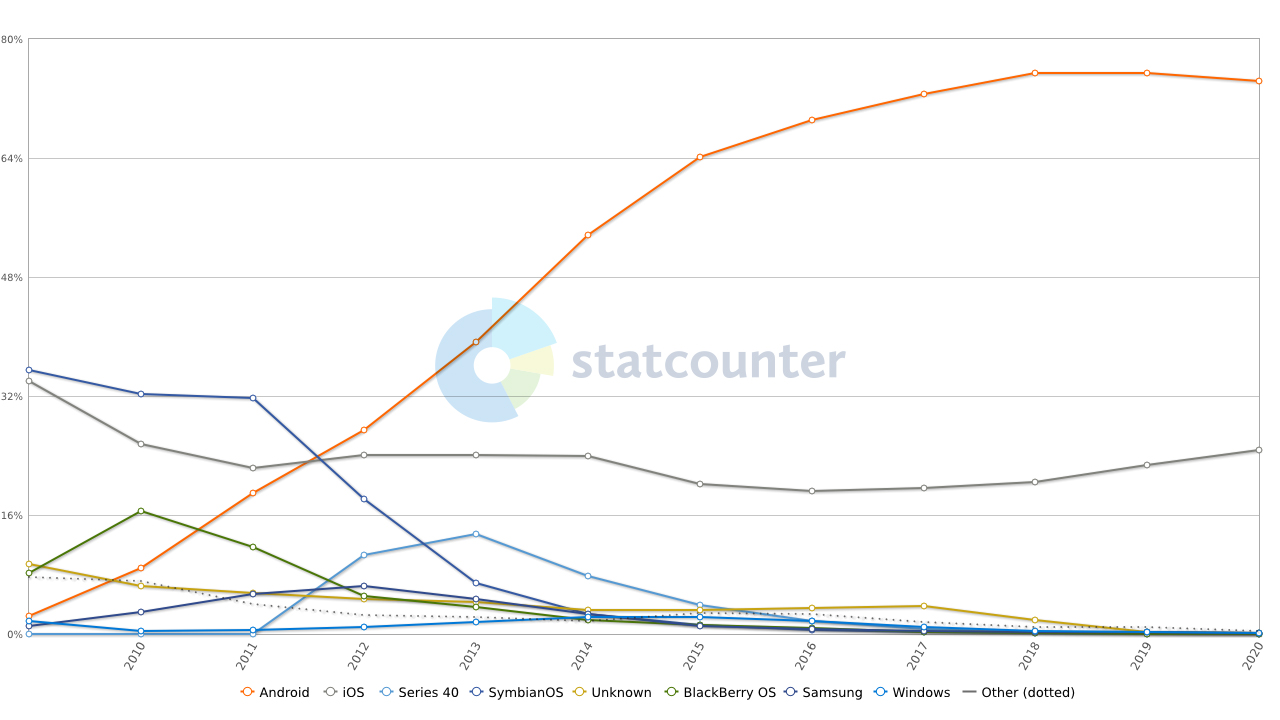
\includegraphics[width=0.95\textwidth]{./Figures/edwin-StatCounter-os-mkt-share-yearly-2009-2020.jpg}
	\caption{2009至2020年移动端操作系统市场份额变化图}
	\label{fig:Android-Mkt-Share}
	\vspace{-5mm}
\end{figure}

\autoref{fig:Android-Mkt-Share}展现了2009年到2020年间不同移动端操作系统对市场占有率的变化曲线,图表来源于数据分析机构StatCounter~\cite{MobileOSMktShare},图表X轴为时间线,Y轴为市场份额占总量的百分比。
不同颜色的曲线代表不同操作系统,其中Android系统由橘红色曲线表示。
从图中数据可知,自发布以来,Android系统便一路高歌猛进,迅速占据移动端操作系统市场,从2012年起就获得了业界第一的市场份额占有率,直到2020年,其超过70\%的市场占有率依然遥遥领先于其他操作系统。
其中原因,除了对用户非常友好的操作方式以外,也在于其具有一个多元、开放又充满活力的应用程序生态环境。

\section{Android应用程序}

\subsection{应用程序简介}

Android应用程序(Android Application,简称App\footnote{App和应用程序/应用三者在Android领域中指代的是同一事物,在本文中可以相互替换,不作区分})是可以安装在Android系统上、拓展系统功能的软件,这些软件通常基于Java语言开发,其中可以包含用C语言或者C++编写的库以提高性能。
2014年起,Google宣布Android支持Kotlin编程语言,自此开发者也可以使用Kotlin语言进行Android App开发。

Android App的开发需要使用Google提供的软件开发工具包(Software Develop Kit,简称SDK)和Google支持的集成开发环境(Integrated Development Environment,简称IDE)。
SDK是包含了众多软件包的工具箱,其中有包括了Android系统应用程序接口(Application Programming Interface,简称API)的函数库和用以编译App的各种工具,在编译完成之后,开发者还可以利用SDK的相应工具为App签上自己的数字签名。
API函数库提供了Android系统的一系列接口,开发者需要在使用Android App框架的前提下,调用各种API实现自己设计的功能。

在发布每一版本Android系统的同时,Google公司也会发布一个新版本的Android SDK供开发者开发App。
每个人都可以从Android的官方网站上下载Android SDK和开发应用所需的IDE,这意味着,利用官方发布的工具,任何人都可以开发出属于自己的Android App。

\subsection{构建应用程序}

与大部分软件一样,开发者在发布自己的App之前,也先需要把代码编译打包成Android操作系统使用的一种应用程序包格式文件APK(Android application package)。
每个APK文件都会包含该款App的一系列基本信息,包括App的应用名、包名(Package name)、安全证书等。
其中,包名是Android系统识别App的依据,每款App在不同的版本可以有不同的应用名,但其包名必须是一致的。
\autoref{fig:Android-Build-Process}展现了APK文件的构建流程。
一般来说,一个Android App的构建流程会分为以下四步,整个构建流程由Android SDK中的Android插件和Gradle构建工具管理。

\begin{figure}[htbp]
	\centering
	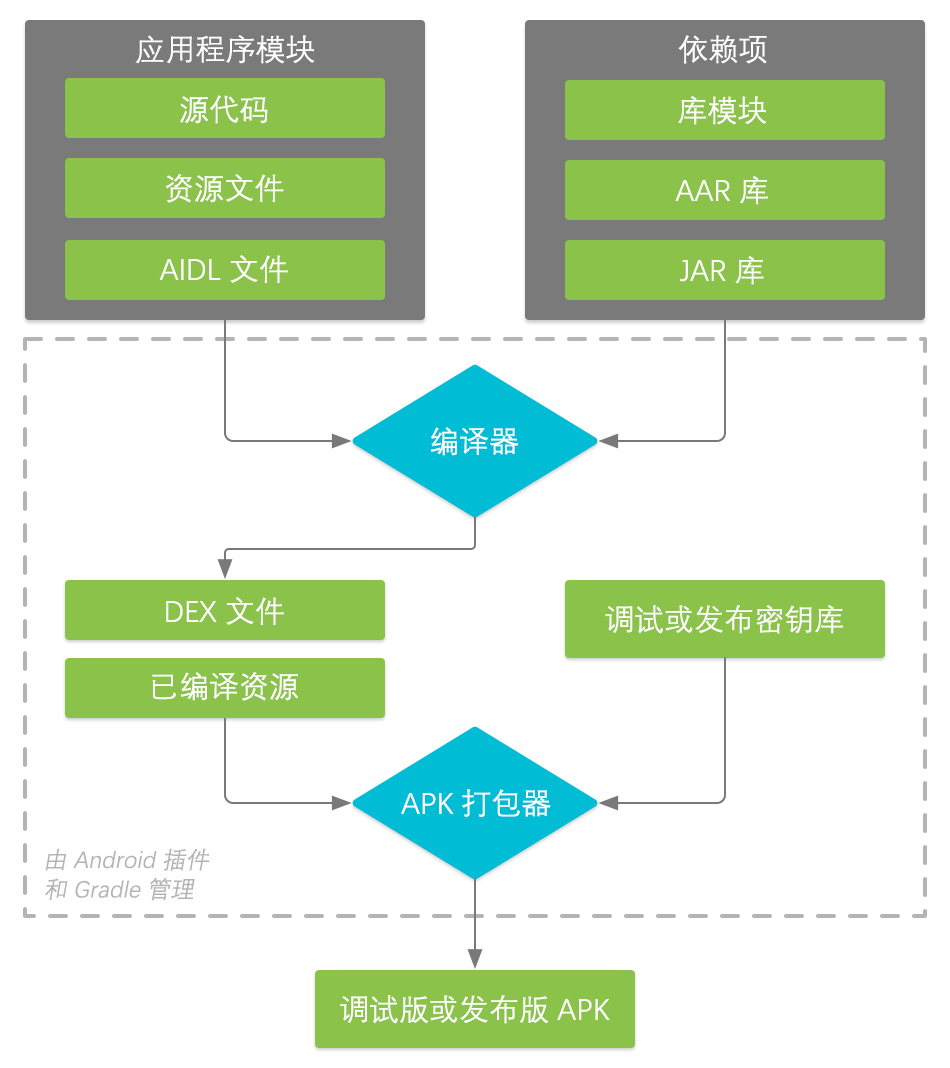
\includegraphics[width=0.6\textwidth]{./Figures/edwin-build-process-CHN.png}
	\caption{Android App构建流程}
	\label{fig:Android-Build-Process}
\end{figure}

首先,开发者需要编写App对应的源代码,然后连同一些源代码中使用到的依赖项一起输入到编译器中生成DEX文件。
源代码可以由Java语言或者Kotlin语言编写,而DEX文件则是一种可执行文件,可以运行于Dalvik虚拟机上。
Dalvik虚拟机则是Android系统的核心组成部分之一,用于运行被编译为DEX文件的程序。
此外,编译器还会将其他未被编译的资源文件转换为编译后的资源。

然后,SDK中的APK打包器会将DEX文件和已经编译好的资源文件一起打包。
APK文件的本质是压缩文件,其中包含了被编译的代码文件、App需要用到的资源文件(比如字符串、图片等资源)、assets资源、App的安全证书和Manifest配置文件,所以APK打包器的任务是将这些所有文件都压缩进一个APK文件里面。
不过,在这个步骤,APK打包器还未将所有文件压缩。
因为在压缩之前,还需要进行下一步的签名。

在第三步,APK打包器会使用密钥库文件对上一步中提及的资源文件和代码文件进行数字签名。
这个步骤是用作校验APK文件是否被篡改、保证APK文件完整性的一个重要步骤,在本章后续内容中会有相关机制的更多介绍。

最后,APK打包器会使用zipalign工具对应用进行优化,以减少App在设备上运行时所占用的内存。
这步结束之后,整个构建流程也随之结束。
开发者会获得一个编译好、签名完毕并且经过优化的APK压缩文件,然后就可以将这个APK文件安装到Android设备上运行使用。


\section{Android应用市场}
\label{sec:androidMkt}
由于每个人都可以开发、构建自己的Android App,从网上发布的App数不胜数。这种开放性为Android应用生态带来开放性的同时,也会引入以下几个问题:

1)\ \emph{难以择优} \quad
开放的环境会导致App数量难以胜数。由于从互联网上找到的App质量良莠不齐,用户有时无法判断网上的应用是否符合自己的需求;

2)\ \emph{数据安全} \quad
智能手机与现代人的日常生活息息相关,其中也自然包含了各人的隐私数据甚至财产信息。确保用户下载、安装到的应用不会损害到他们的财产安全和数据安全至关重要;

3)\ \emph{宣传渠道} \quad
开发者希望自己的App尽可能地受欢迎,但中小开发者并没有足够的资源去宣传自己的应用,可能会导致原本质量优秀的App因为缺少宣传渠道而无人问津;

4)\ \emph{收入结算} \quad
开发者有从App中获得盈利的需求。即使是部分出于兴趣或其他非盈利目的开发手机应用的开发者,也需要从App中获取补贴以维持App的维护和正常运作。如何利用App变现、变现之后又要怎样将资金回流到开发者的问题有待解决;

5)\ \emph{应用更新} \quad
随着时间推进,用户的需求并非一成不变,开发者也需要针对App中以往出现的漏洞查漏补缺、或者更新软件功能,但要求用户定期/不定期地手动更新某个App甚至多个App并不现实。

Google发布的应用商店Google Play~\cite{GooglePlay}的存在缓解了以上的问题。它是Android操作系统的官方应用商店,可以让用户浏览和下载商店中的App。
一方面,普通用户可以经由Android系统中预装好的Google Play服务寻找、购买和下载心仪的App;另一方面,Google Play也允许开发者将App通过开发者账户上传到Google Play中,在经过一系列的审查之后上架到商场上供用户下载。与上述的五个问题对应,Google Play应用商店提供了以下几点服务:

1)\ \emph{一个由官方背书的下载渠道} \quad
这确保了用户下载的App得到官方认可。同时,Google Play也提供了一个关于App的社区环境,用户可以对App进行打分、评论,用户对App的评价经审核后可以由所有其他用户查看,直接影响其他用户对``是否要下载某款应用''的决定;

2)\ \emph{上架之前的应用审核} \quad
在开发者上传App时对App作出一定的审查,以排除部分恶意开发者在商场中上架病毒和恶意应用的可能性。Google Play也会根据用户反馈、应用本身运营数据等原因于每季度从商店中移除一部分App,以保证商店货架上App的质量;

3)\ \emph{作为激励机制的推荐榜单} \quad
在用户评价的基础上,Google Play筛选出一部分质量优异的App制订出一些推荐榜单。推荐榜单会在应用商店首页进行展示,榜单包括``编辑精选''、``热门应用''、``年度之选''等,其中既有大公司开发的App,也会有中小开发者独立开发的应用。此外,Google还会通过用户的使用习惯、所在地区等因素为用户提供个性化推荐(如\autoref{fig:Google-Play-Main}所示),在不同的App类别下,也有不同榜单为用户推荐,加大了优秀App的曝光率;

\begin{figure}[htbp]
	\centering
	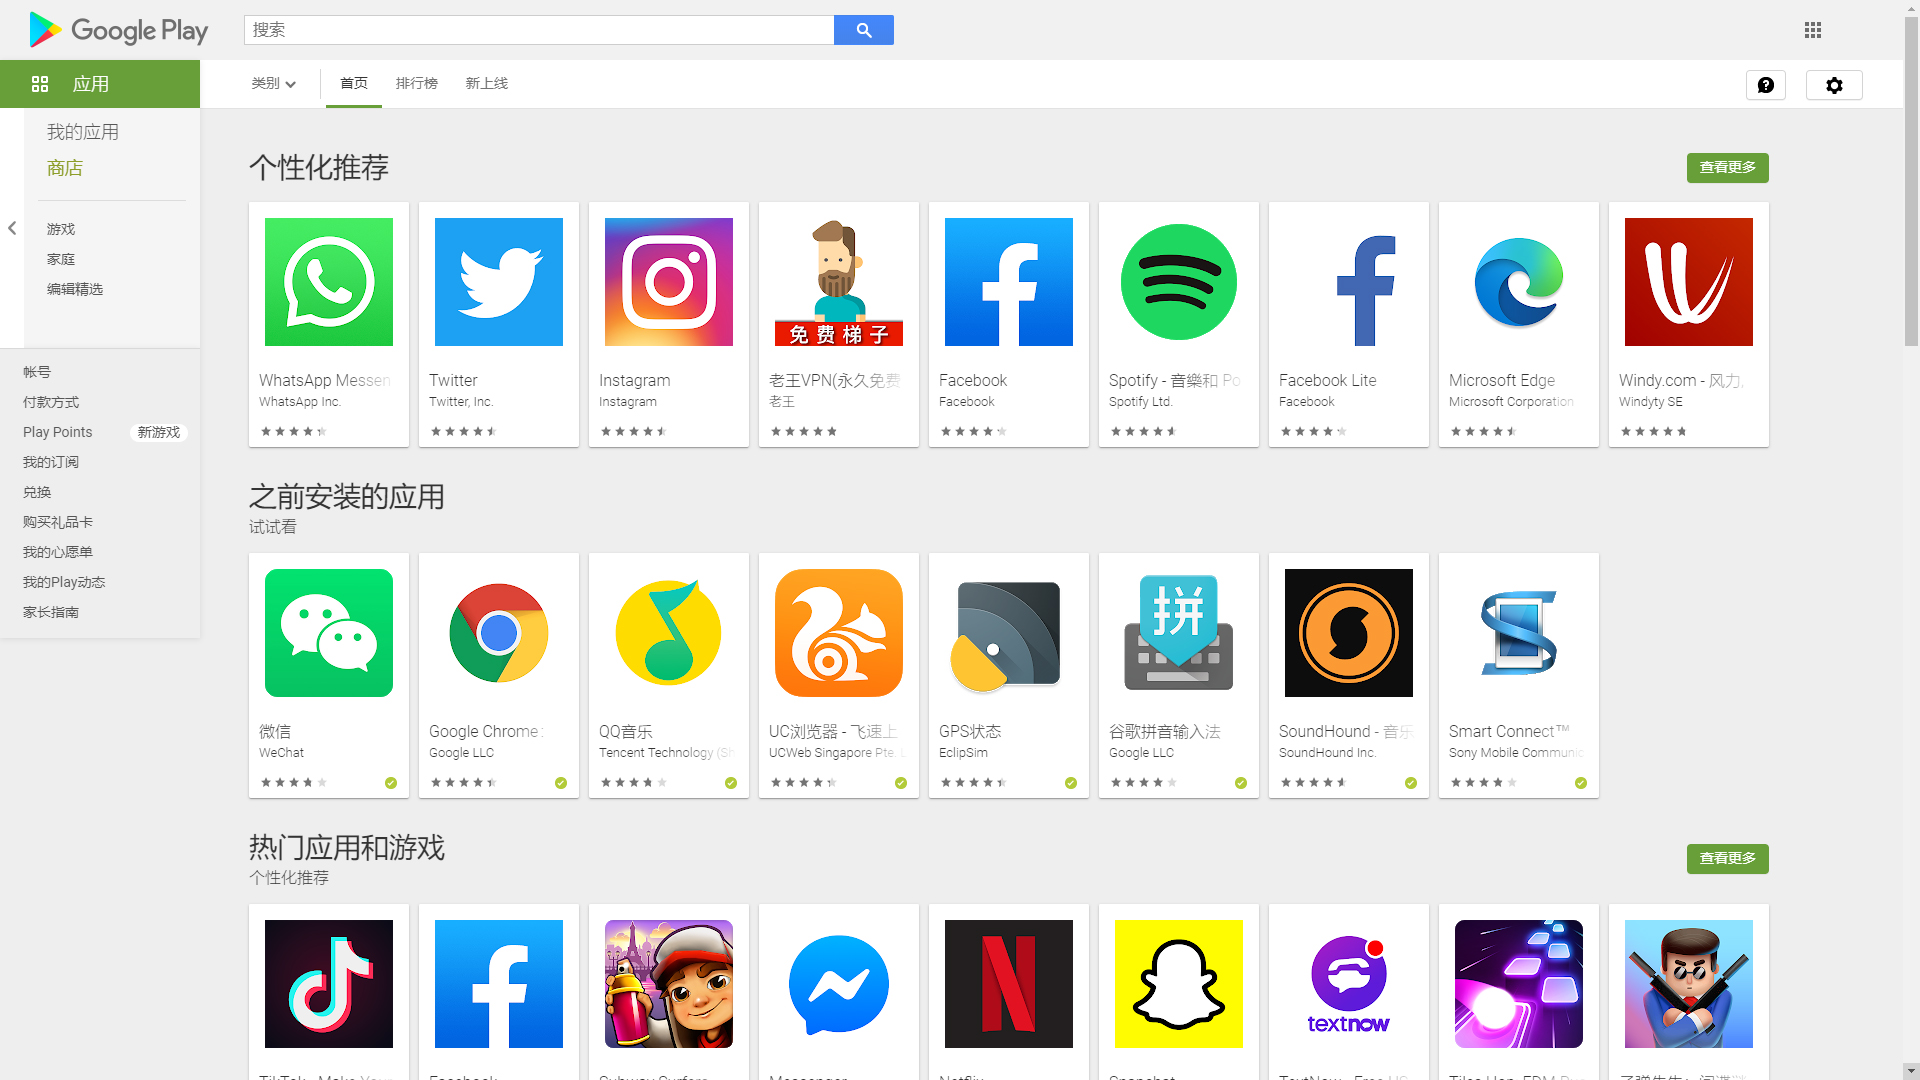
\includegraphics[width=\textwidth]{./Figures/edwin-google-play.jpg}
	\caption{Google Play应用商店首页(从桌面端浏览)}
	\label{fig:Google-Play-Main}
\end{figure}

4)\ \emph{集中的结算通道} \quad
Google Play应用商店为开发者提供了一个统一的结算渠道。应用开发者可以在App内销售商品,然后选择Google Play提供的集成结算服务。用户在购买服务时,直接向Google付款,Google再在每个结算周期将款项结算给开发者。这样一来,开发者尤其是独立开发者就可以更专注于App本身的开发,而不需要考虑如何利用应用变现、再将资金回收的复杂问题。Google Play也允许开发者将自己的App上架为付费应用,需要用户付款后才可下载;

5)\ \emph{方便快捷的更新推送} \quad
由于Google Play本身是个应用程序的集中平台,而且也预置到了大多搭载Android的设备中,所以开发者在更新应用时,只需将新版本上传到Google Play的后台,应用商店经过审核之后,就可以将新版本的应用推送到用户的设备中,让用户设备中的App实现自动更新,免去双方的麻烦。


\section{第三方应用市场}

Google Play应用商店无疑为用户和开发者都提供了一个优良的解决方案,每个应用底下由用户评论组成的社区也促成了用户和开发者之间的交流,用户反馈直接推动了开发者对应用的改良。

遗憾的是,由于种种原因,Google Play应用商店的服务并非对全球的所有地区和国家都开放。
Google从2008年开始退出中国大陆市场,因此Google的大部分服务,包括Google Play应用商店的下载服务在内,都不向中国大陆境内用户提供。
换句话说,国内的大部分普通用户并不能享受到Google Play应用商店的便利。

为此,国内有多家厂商都推出了自己开发的应用市场服务,试图填补这一片市场空白。
实际上,由于整合开发者、用户和App资源三者本身就有巨大的市场潜力,所以即使是在Google Play服务可用的其他国家和地区,也有厂商推出自己的应用市场(如三星推出的三星应用商店、Amazon推出的Amazon应用市场),试着在这个市场上分一杯羹。

纵观国内的应用市场,经过几年的竞争与整合,依然未有出现像Google Play应用商店一样具有垄断性地位的厂商。
多个厂商各据一方,主要可以分为两个类别。
一类是国内IT行业巨头旗下的应用市场,如腾讯旗下的应用宝~\cite{Myapp}和百度旗下的百度应用市场~\cite{Baiduappstore},其平台本身就具有大量基础用户,可以直接转化为应用市场中的活跃用户;另一类则是由各大手机厂商开发的应用市场,如华为的应用市场、小米的小米应用市场~\cite{Xiaomiappstore}等,这类的应用市场通常直接预装在手机出厂时自带的厂家定制Android系统中,凭借手机销量直接带动市场用户增长。

根据数据分析机构艾媒咨询于2018年12月发布的《2018-2019中国中国移动应用商店市场监测报告》~\cite{ChineseAppStoreReport}显示,使用第三方移动应用商店的用户在手机网民中占比为59.99\%。结合国内网民数目庞大的现状,这一数字表示第三方应用市场在国内已被广泛接受。而40.01\%未使用第三方移动应用商店的用户比例则表示这一市场还有广阔前景。该报告还提供了2018年国内第三方应用市场用户首选市场的分布图,如\autoref{fig:CHN-Mkt-Dist}所示,用户对第三方移动应用市场的选择主要还是集中在国内IT巨头发布的应用市场上。约40\%的手机用户会使用360旗下的360手机助手作为首选应用市场,而首选使用豌豆荚、UC应用商店等阿里应用分发平台旗下应用商店的用户约占11\%。大部分市场份额都已被国内IT巨头旗下的应用市场占领。

\begin{figure}[htbp]
	\centering
	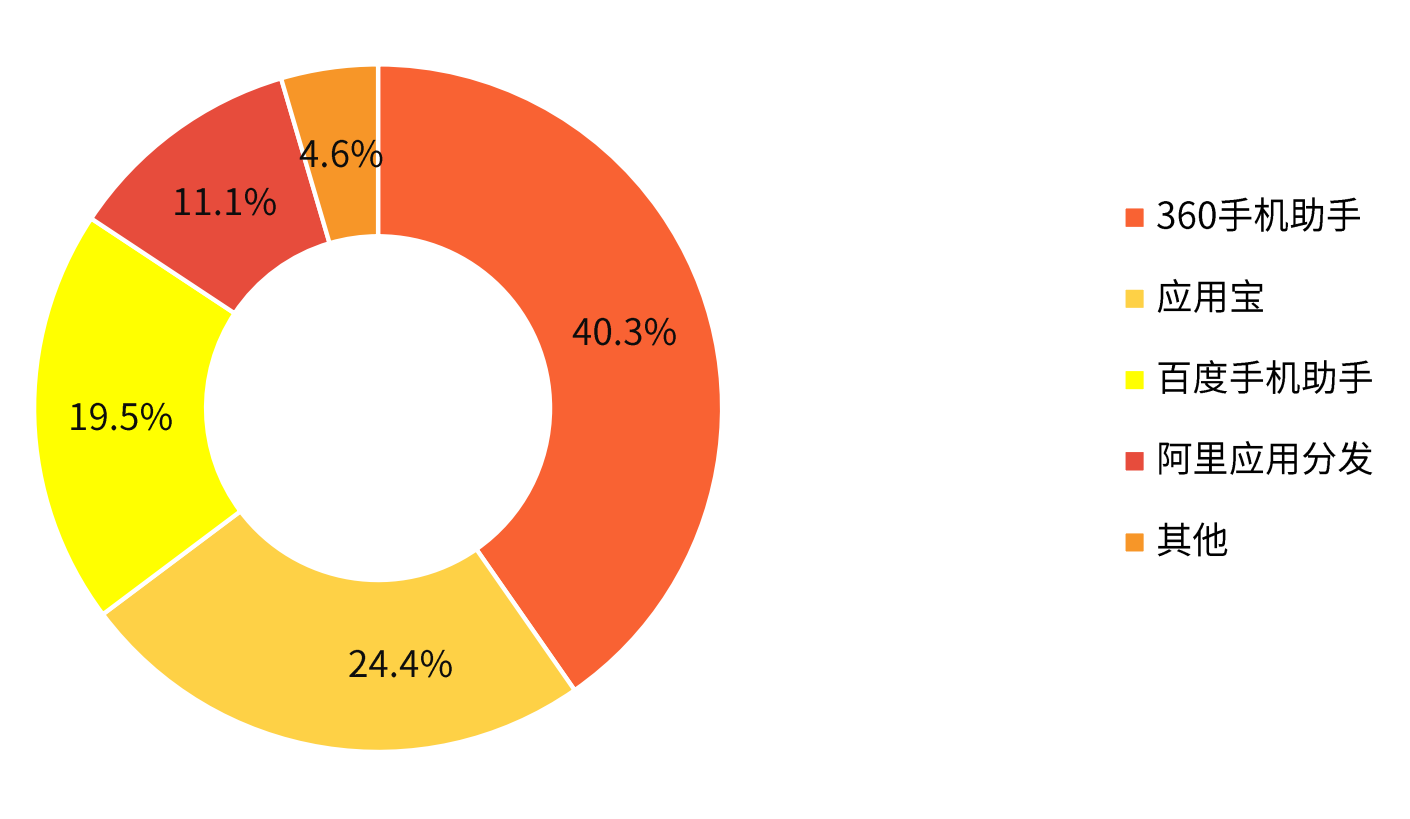
\includegraphics[width=0.5\textwidth]{./Figures/edwin-CHN-mkt-dist.png}
	\caption{2018中国第三方移动应用商店用户首选使用品牌分布}
	\label{fig:CHN-Mkt-Dist}
\end{figure}

与Google Play提供一个完整的Android生态环境相似,上述的各个厂商也致力于构建各自的Android应用生态链条:各大厂商本身就具有一定知名度,从其旗下的应用市场下载应用能让用户放心;开放开发者中心,让开发者注册账号后上传自己制作的App;为每一个App提供评分和评论功能,构建出开发者和用户的交流平台;在应用市场首页设置应用排行榜、推荐安装软件等榜单(如\autoref{fig:mkt-yyb}),提高优秀App的曝光率;应用市场自带的应用版本管理开发者在市场后台更新应用之后,将更新推送到用户的手机上;各大应用市场也会整合支付平台(如支付宝和微信支付)来应对市场内的应用购买业务,华为应用市场甚至像Google Play一样,为市场上的应用提供了自家的支付渠道以支持应用内的付款项目购买功能。

\begin{figure}[htbp]
	\centering
	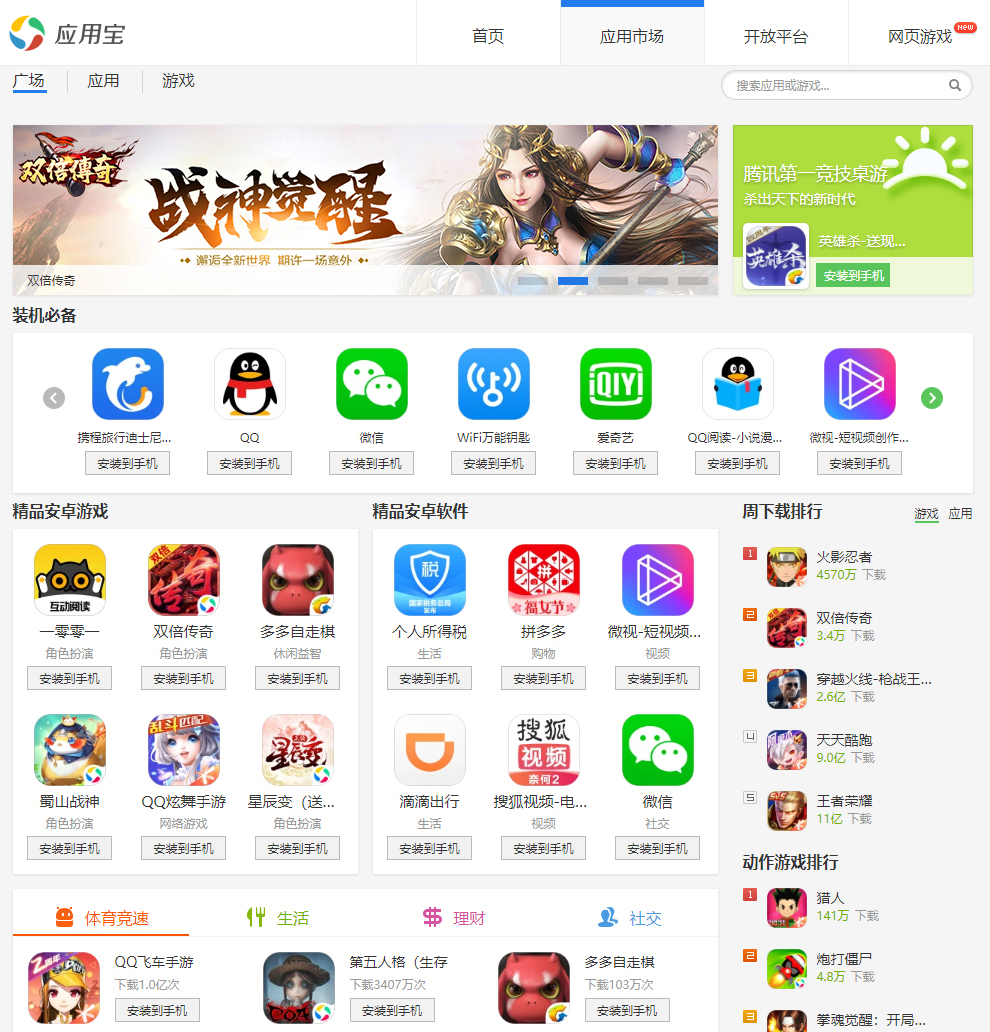
\includegraphics[width=0.8\textwidth]{./Figures/edwin-yyb.jpg}
	\caption{腾讯应用宝应用市场首页(从桌面端浏览)}
	\label{fig:mkt-yyb}
	\vspace{-5mm}
\end{figure}

不同于在Android系统发布早期就存在的Google Play应用商店,国内的第三方应用商店是后期出现的产物,一出现就面临着激烈的市场竞争。
一方面,在国内各类第三方应用市场方兴未艾之时,国内的Android开发者社群尚未成熟,应用市场还未有大量开发者进驻;
另一方面,在成立初期,为了抢占市场份额,各个应用商店都想方设法将商店内App的种类和数量最大化,以迎合市场用户各种各样的需求。
作为结果,各类第三方应用市场都在各个渠道搜集App,而非通过开发者上传的方式获得货架上的应用程序。
由于在早期各种监管渠道尚未完善,各个市场在搜罗各类App的同时,难免会将大量的盗版应用也一并收录。

\section{Android App签名机制}
\label{sec:signature}

前文提到,开发者在使用Android SDK构建App时,其中十分重要的一步是对App进行数字签名。
实际上,Android的数字签名和安全证书机制基于RSA公共密钥系统,是Android安全机制中不可或缺的一个部分。
本章的余下内容将会对Android App的签名机制进行简单分析。

Android App的签名机制是用作校验APK文件是否被篡改、保证APK文件完整性的一个重要机制,所有的应用都必须要在经过签名才能安装进Android系统中。
在签名时,SDK会使用一种密钥库文件,如果开发者还没有这个文件的话,SDK会自动生成一个。
密钥库中包含了开发者的各种信息,包括一对公钥和私钥。
私钥用于数字签名,不可向外公布;公钥则是可以向外公布的一组密钥,用于数字前面的验证。
App中的签名也是系统用来识别开发者的重要依据,因为同一个密钥库文件会产生一致的签名,系统能根据签名中的公钥验证应用识别开发者。

签名的过程大致如下:
在前文流程的第二步结束后,编译器会输出DEX文件和编译好的资源文件,这时,SDK会对每个文件都扫描一次,然后对每个文件提取一次数字摘要,再把每个文件的文件名和其对应的数字摘要保存在一个名为\textit{MANIFEST.MF}的文件中。
之后,SDK会再扫描一次刚才生成的\textit{MANIFEST.MF}文件,再次提取一次数字摘要,把这个摘要连同刚才文件中的所有内容存入另一个新文件\textit{CERT.SF}里。
第三步,再计算一次\textit{CERT.SF}的数字摘要,然后用密钥库中的私钥对这个摘要进行加密。
加密后的结果就是数字签名。
最后,SDK将签名、公钥、计算数字摘要的哈希算法等信息写入\textit{CERT.RSA}文件中,再将这整个过程中生成的四个文件放进\textit{META-INF}文件夹,用APK打包器打包起来。
至此流程结束。

而Android系统验证签名的方式,则是先通过\textit{CERT.RSA}中的公钥验证签名是否无误,再根据文件中提供的哈希算法计算APK包中所有文件的数字摘要:先从\textit{CERT.SF}开始,然后是\textit{MANIFEST.MF},然后是APK中的其他所有文件...
一旦其中出现不相符的结果,就会导致验证失败。
在安装App的过程中,验证签名失败会使得系统终止App的安装。

换句话说,在一个APK被打包签名完毕之后,如果需要更改其中的内容,就只能在更改后将APK重新打包签名一次,即使是一个bit的修改也会破坏原有的签名。
这也是系统可以用数字签名识别开发者的原因:签名一致的App,最后一定都是由同一个开发者打包的。
所以,具有同样签名的App也可以在同一个Android设备上共享数据。
不过这超出了本文讨论的内容,故按下不表。

目前,签名的模式共有三代,其区别主要在于构建流程第三、第四步之间的一些操作上。
简单地说,越新的签名模式能越好地保障APK文件的完整性。
实际上,第一代签名模式V1具有较为致命的缺陷,所以Google官方也在呼吁开发者在编译时采用最新的签名模式。

要注意的是,签名机制只能保证APK文件在被篡改之后不能凭借原有的签名被安装进Android系统,但恶意开发者依然可以在篡改APK之后,用自己的密钥库对APK重新签名,构建出可安装的App。
这种App是盗版App的一种,被称为重打包App。

另外,虽然一个安全证书只能指向一名开发者,但一个开发者可以同时拥有多个安全证书。
开发者和安全证书之间具有一对多的映射关系。

\section{本章小结}

本章主要介绍了Android系统、Android应用和Android应用市场的相关背景知识,同时也阐述了Android应用的构建流程和简要介绍了其中使用到的签名机制,为后文实证研究中使用到的采样来源和验证方法做铺垫。
